\documentclass[a4paper, 12pt]{article}

%% Language and font encodings
\usepackage[english]{babel}
\usepackage[utf8]{inputenc}
\usepackage[T1]{fontenc}

%% Sets page size and margins
\usepackage[a4paper,top=2cm,bottom=2cm,left=3cm,right=3cm,marginparwidth=1.75cm]{geometry}

%% Useful packages
\usepackage[tbtags]{amsmath}
\usepackage{mathtools}
\usepackage[colorlinks=true, allcolors=blue]{hyperref}
\usepackage{color}
\usepackage{caption}
\usepackage[shortlabels]{enumitem}
\usepackage{authblk}
\usepackage{xr}

% package to manage citations
\usepackage[backend=bibtex,style=authoryear-comp,sorting=nyt,isbn=false,url=false, natbib=true, doi=false]{biblatex}
\addbibresource{bibliography.bib}

\newcommand*\diff{\mathop{}\!\mathrm{d}}
%\newcommand{\argmax}[1]{\underset{#1}{\operatorname{arg}\,\operatorname{max}}\;}
\DeclareMathOperator{\argmax}{arg\,max}
\DeclarePairedDelimiter\abs{\lvert}{\rvert}%
\DeclarePairedDelimiter\norm{\lVert}{\rVert}%

\newcommand{\Hline}
{
\hline
\hline
}

\renewcommand{\thesection}{Web Appendix \Alph{section}}
\makeatletter
\renewcommand{\fnum@figure}{Web Figure \thefigure}
\makeatother

\AtBeginDocument{%
	\renewcommand{\thetable}{Web Table \arabic{table}}
}

\begin{document}
\title{\textbf{Supplementary Materials for ``Personalized Schedules for Burdensome Surveillance Tests''}}

\author[1,*]{\normalsize Anirudh Tomer}
\author[2,3]{Daan Nieboer}
\author[3]{Monique J. Roobol}
\author[2,4]{Ewout W. Steyerberg}
\author[1]{Dimitris Rizopoulos}
\affil[1]{Department of Biostatistics, Erasmus University Medical Center, the Netherlands}
\affil[2]{Department of Public Health, Erasmus University Medical Center, the Netherlands}
\affil[3]{Department of Urology, Erasmus University Medical Center, the Netherlands}
\affil[4]{Department of Biomedical Data Sciences, Leiden University Medical Center, the Netherlands}
\affil[ ]{*\textit {email}: a.tomer@erasmusmc.nl}

\date{}

\maketitle

% !TEX root =  ../supplementary.tex
\section{Joint Model for Time-to-Event and Longitudinal Outcomes}
\label{web_sec : jm_framework}
We start with a short introduction of the joint modeling framework we will use in our following developments. Let $T_i^*$ denote the true Gleason reclassification (GR) time for the $i$-th patient and let $S$ be the schedule of his biopsies. Let the vector of the time of biopsies be denoted by $T_i^S = \{T^S_{i0}, T^S_{i1}, \ldots, T^S_{i{N_i^S}}; T^S_{ij} < T^S_{ik}, \forall j<k\}$, where $N_i^S$ are the total number of biopsies conducted. Because biopsy schedules are periodical, $T_i^*$ cannot be observed directly and it is only known to fall in an interval $l_i < T_i^* \leq r_i$, where $l_i = T^S_{i{N_i^S - 1}}, r_i = T^S_{i{N_i^S}}$ if GR is observed, and $l_i = T^S_{i{N_i^S}}, r_i=\infty$ if GR is not observed yet. Further let $\bmath{y}_i$ denote the $n_i \times 1$ vector of prostate-specific antigen (PSA) levels for the $i$-th patient. For a sample of $n$ patients the observ{}ed data is denoted by $\mathcal{D}_n = \{l_i, r_i, \bmath{y}_i; i = 1, \ldots, n\}$.

The longitudinal outcome of interest, namely PSA level, is continuous in nature and thus to model it the joint model utilizes a linear mixed effects model (LMM) of the form:
\begin{equation*}
\begin{split}
y_i(t) &= m_i(t) + \varepsilon_i(t)\\
&=\bmath{x}_i^T(t) \bmath{\beta} + \bmath{z}_i^T(t) \bmath{b}_i + \varepsilon_i(t),
\end{split}
\end{equation*}
where $\bmath{x}_i(t)$ and $\bmath{z}_i(t)$ denote the row vectors of the design matrix for fixed and random effects, respectively. The fixed and random effects are denoted by $\bmath{\beta}$ and $\bmath{b}_i$, respectively. The random effects are assumed to be normally distributed with mean zero and $q \times q$ covariance matrix $\bmath{D}$. The true and unobserved, error free PSA level at time $t$ is denoted by $m_i(t)$. The error $\varepsilon_i(t)$ is assumed to be t-distributed with three degrees of freedom and scale $\sigma$ (see \ref{subsec : t_dist_choice}), and is independent of the random effects $\bmath{b}_i$.

To model the effect of PSA on hazard of GR, joint models utilize a relative risk sub-model. The hazard of GR for patient $i$ at any time point $t$, denoted by $h_i(t)$, depends on a function of subject specific linear predictor $m_i(t)$ and/or the random effects:
\begin{align*}
h_i(t \mid \mathcal{M}_i(t), \bmath{w}_i) &= \lim_{\Delta t \to 0} \frac{\mbox{Pr}\big\{t \leq T^*_i < t + \Delta t \mid T^*_i \geq t, \mathcal{M}_i(t), \bmath{w}_i\big\}}{\Delta t}\\
&=h_0(t) \exp\big[\bmath{\gamma}^T\bmath{w}_i + f\{\mathcal{M}_i(t), \bmath{b}_i, \bmath{\alpha}\}\big], \quad t>0,
\end{align*}
where $\mathcal{M}_i(t) = \{m_i(v), 0\leq v \leq t\}$ denotes the history of the underlying PSA levels up to time $t$. The vector of baseline covariates is denoted by $\bmath{w}_i$, and $\bmath{\gamma}$ are the corresponding parameters. The function $f(\cdot)$ parametrized by vector $\bmath{\alpha}$ specifies the functional form of PSA levels \citep{brown2009assessing,rizopoulos2012joint,taylor2013real,rizopoulos2014bma} that is used in the linear predictor of the relative risk sub-model. Some functional forms relevant to the problem at hand are the following: 
\begin{eqnarray*}
\left \{
\begin{array}{l}
f\{\mathcal{M}_i(t), \bmath{b}_i, \bmath{\alpha}\} = \alpha m_i(t),\\
f\{\mathcal{M}_i(t), \bmath{b}_i, \bmath{\alpha}\} = \alpha_1 m_i(t) + \alpha_2 m'_i(t),\quad \text{with}\  m'_i(t) = \frac{\rmn{d}{m_i(t)}}{\rmn{d}{t}}.\\
\end{array}
\right.
\end{eqnarray*}
These formulations of $f(\cdot)$ postulate that the hazard of GR at time $t$ may be associated with the underlying level $m_i(t)$ of the PSA at $t$, or with both the level and velocity $m'_i(t)$ of the PSA at $t$. Lastly, $h_0(t)$ is the baseline hazard at time $t$, and is modeled flexibly using P-splines. More specifically:
\begin{equation*}
\log{h_0(t)} = \gamma_{h_0,0} + \sum_{q=1}^Q \gamma_{h_0,q} B_q(t, \bmath{v}),
\end{equation*}
where $B_q(t, \bmath{v})$ denotes the $q$-th basis function of a B-spline with knots $\bmath{v} = v_1, \ldots, v_Q$ and vector of spline coefficients $\gamma_{h_0}$. To avoid choosing the number and position of knots in the spline, a relatively high number of knots (e.g., 15 to 20) are chosen and the corresponding B-spline regression coefficients $\gamma_{h_0}$ are penalized using a differences penalty \citep{eilers1996flexible}.

\clearpage

\subsection{Parameter Estimation}
We estimate parameters of the joint model using Markov chain Monte Carlo (MCMC) methods under the Bayesian framework. Let $\bmath{\theta}$ denote the vector of the parameters of the joint model. The joint model postulates that given the random effects, time to GR and longitudinal responses taken over time are all mutually independent. Under this assumption the posterior distribution of the parameters is given by:
\begin{align*}
p(\bmath{\theta}, \bmath{b} \mid \mathcal{D}_n) & \propto \prod_{i=1}^n p(l_i, r_i, \bmath{y}_i \mid \bmath{b}_i, \bmath{\theta}) p(\bmath{b}_i \mid \bmath{\theta}) p(\bmath{\theta})\\
& \propto \prod_{i=1}^n p(l_i, r_i \mid \bmath{b}_i, \bmath{\theta}) p(\bmath{y}_i \mid \bmath{b}_i, \bmath{\theta}) p(\bmath{b}_i \mid \bmath{\theta}) p(\bmath{\theta}),\\
p(\bmath{b}_i \mid \bmath{\theta}) &= \frac{1}{\sqrt{(2 \pi)^q \text{det}(\bmath{D})}} \exp(\bmath{b}_i^T \bmath{D}^{-1} \bmath{b}_i),
\end{align*}
where the likelihood contribution of longitudinal outcome conditional on random effects is:
\begin{align*}
p(\bmath{y}_i \mid \bmath{b}_i, \bmath{\theta}) &= \frac{1}{\big(\sqrt{2 \pi \sigma^2}\big)^{n_i}} \exp\bigg(-\frac{{\lVert{\bmath{y}_i - \bmath{X}_i\bmath{\beta} - \bmath{Z}_i\bmath{b}_i}\rVert}^2}{\sigma^2}\bigg),\\
\bmath{X}_i &= \{\bmath{x}_i(t_{i1})^T, \ldots, \bmath{x}_i(t_{in_i})^T\}^T,\\
\bmath{Z}_i &= \{\bmath{z}_i(t_{i1})^T, \ldots, \bmath{z}_i(t_{in_i})^T\}^T.
\end{align*}
The likelihood contribution of the time to GR outcome is given by:
\begin{equation}
\label{web_eq : likelihood_contribution_survival}
p(l_i,r_i\mid \bmath{b}_i,\bmath{\theta}) = \exp\Big\{-\int_0^{l_i} h_i(s \mid \mathcal{M}_i(s), \bmath{w}_i)\rmn{d}{s}\Big\} - \exp\Big\{-\int_0^{r_i}h_i(s \mid \mathcal{M}_i(s), \bmath{w}_i)\rmn{d}{s}\Big\}.
\end{equation}
The integral in (\ref{web_eq : likelihood_contribution_survival}) does not have a closed-form solution, and therefore we use a 15-point Gauss-Kronrod quadrature rule to approximate it.

We use independent normal priors with zero mean and variance 100 for the fixed effects $\bmath{\beta}$, and inverse Gamma prior with shape and rate both equal to 0.01 for the parameter $\sigma^2$. For the variance-covariance matrix $\bmath{D}$ of the random effects we take inverse Wishart prior with an identity scale matrix and degrees of freedom equal to $q$ (number of random effects). For the relative risk model's parameters $\bmath{\gamma}$ and the association parameters $\bmath{\alpha}$, we use independent normal priors with zero mean and variance 100.

\clearpage
\subsection{Interval Censoring in Time of Gleason Reclassification}
\label{subsec : int_censoring_fulllikelihood_proof}
The true time of GR $T^*_i$ is not known for any of the patients. In order to detect GR, PRIAS uses a fixed schedule of biopsies wherein biopsies are conducted at year one, year four, year seven and year ten of follow-up, and every five years thereafter. However, PRIAS switches to a more frequent annual biopsy schedule for faster-progressing patients. These are patients with PSA doubling time (PSA-DT) of less than 10 years. The latter is measured as the inverse of the slope of the regression line through the base two logarithm of PSA values. Thus, the interval $l_i < T_i^* \leq r_i$ in which GR is detected depends on the observed PSA values. 

It is natural to question in this scenario if the parameters of the joint model are affected by PSA-DT dependent interval censoring. However, because the parameters of the joint model are estimated using a full likelihood approach \citep{tsiatis2004joint}, the joint model allows the schedule of biopsies to depend upon the observed PSA values (e.g., via PSA-DT), under the condition that the model is correctly specified (we discuss this aspect in \ref{sec : param_estimates_jm_fit_prias}). To show this, consider the following full general specification of the joint model that we use. Let $\boldsymbol{y}_i$ denote the observed PSA measurements for the $i$-th patient, and $l_i, r_i$ denote the two time points of the interval in which GR occurs for the $i$-th patient. In addition let $T_i^S$ and $\mathcal{V}_i$ denote the schedule of biopsies and schedule of PSA measurements, respectively. Under the assumption that both of these schedules may depend upon only the observed $\boldsymbol{y}_i$, the joint likelihood of all four processes is given by:
\begin{equation}
p(\boldsymbol{y}_i, l_i, r_i, T_i^S, \mathcal{V}_i \mid \boldsymbol{\theta}, \boldsymbol{\psi}) = p(\boldsymbol{y}_i, l_i, r_i \mid \theta) \times p(T_i^S, \mathcal{V}_i \mid \boldsymbol{y}_i, \boldsymbol{\psi}).
\end{equation}
From this decomposition we can see that even if the processes $T_i^S$ and $\mathcal{V}_i$ may be determined from $\boldsymbol{y}_i$, if we are interested in the parameters $\boldsymbol{\theta}$ of the joint distribution of longitudinal and event outcome, we can maximize the likelihood based on the first term and ignore the second term. In other words, the second term will not carry information for $\boldsymbol{\theta}$.

It is important to note that, since we use a full likelihood approach with an interval censoring specification, the estimates that we obtain are consistent and asymptotically unbiased \citep{gentleman1994maximum}, despite the interval censoring observed. 

\clearpage

\subsubsection{Parameter Estimates}
\label{subsec : param_estimates_jm_fit_prias}
The posterior parameter estimates for the joint model we fitted to the PRIAS dataset are shown in Table \ref{tab : PSA_long} and Table \ref{tab : PSA_survival}. Since the longitudinal evolution of $\log_2 \mbox{PSA}$ is modeled with non-linear terms, the interpretation of the coefficients corresponding to time is not straightforward. In lieu of the interpretation we present the fitted evolution of PSA (Figure \ref{fig : fitted_trend_psa}) over a period of 10 years for a patient who is 70 years old. It can be seen that after the first 6 months the PSA levels steadily increase over the follow up period. Since the model for PSA has only additive terms, this evolution remains same for all patients. The effect of age only affects the baseline PSA score. However it is so small that it can be ignored for all practical purposes.

For the relative risk sub-model, the parameter estimates in Table \ref{tab : PSA_survival} show that only $\log_2 \mbox{PSA}$ velocity is strongly associated with hazard of GR. For any patient, a unit increase in $\log_2 \mbox{PSA}$ velocity corresponds to a 11 time increase in hazard of GR. The effect of $\log_2 \mbox{PSA}$ value and effect of Age on hazard of GR are small enough to be safely ignored for all practical purposes.

\begin{figure}
\centerline{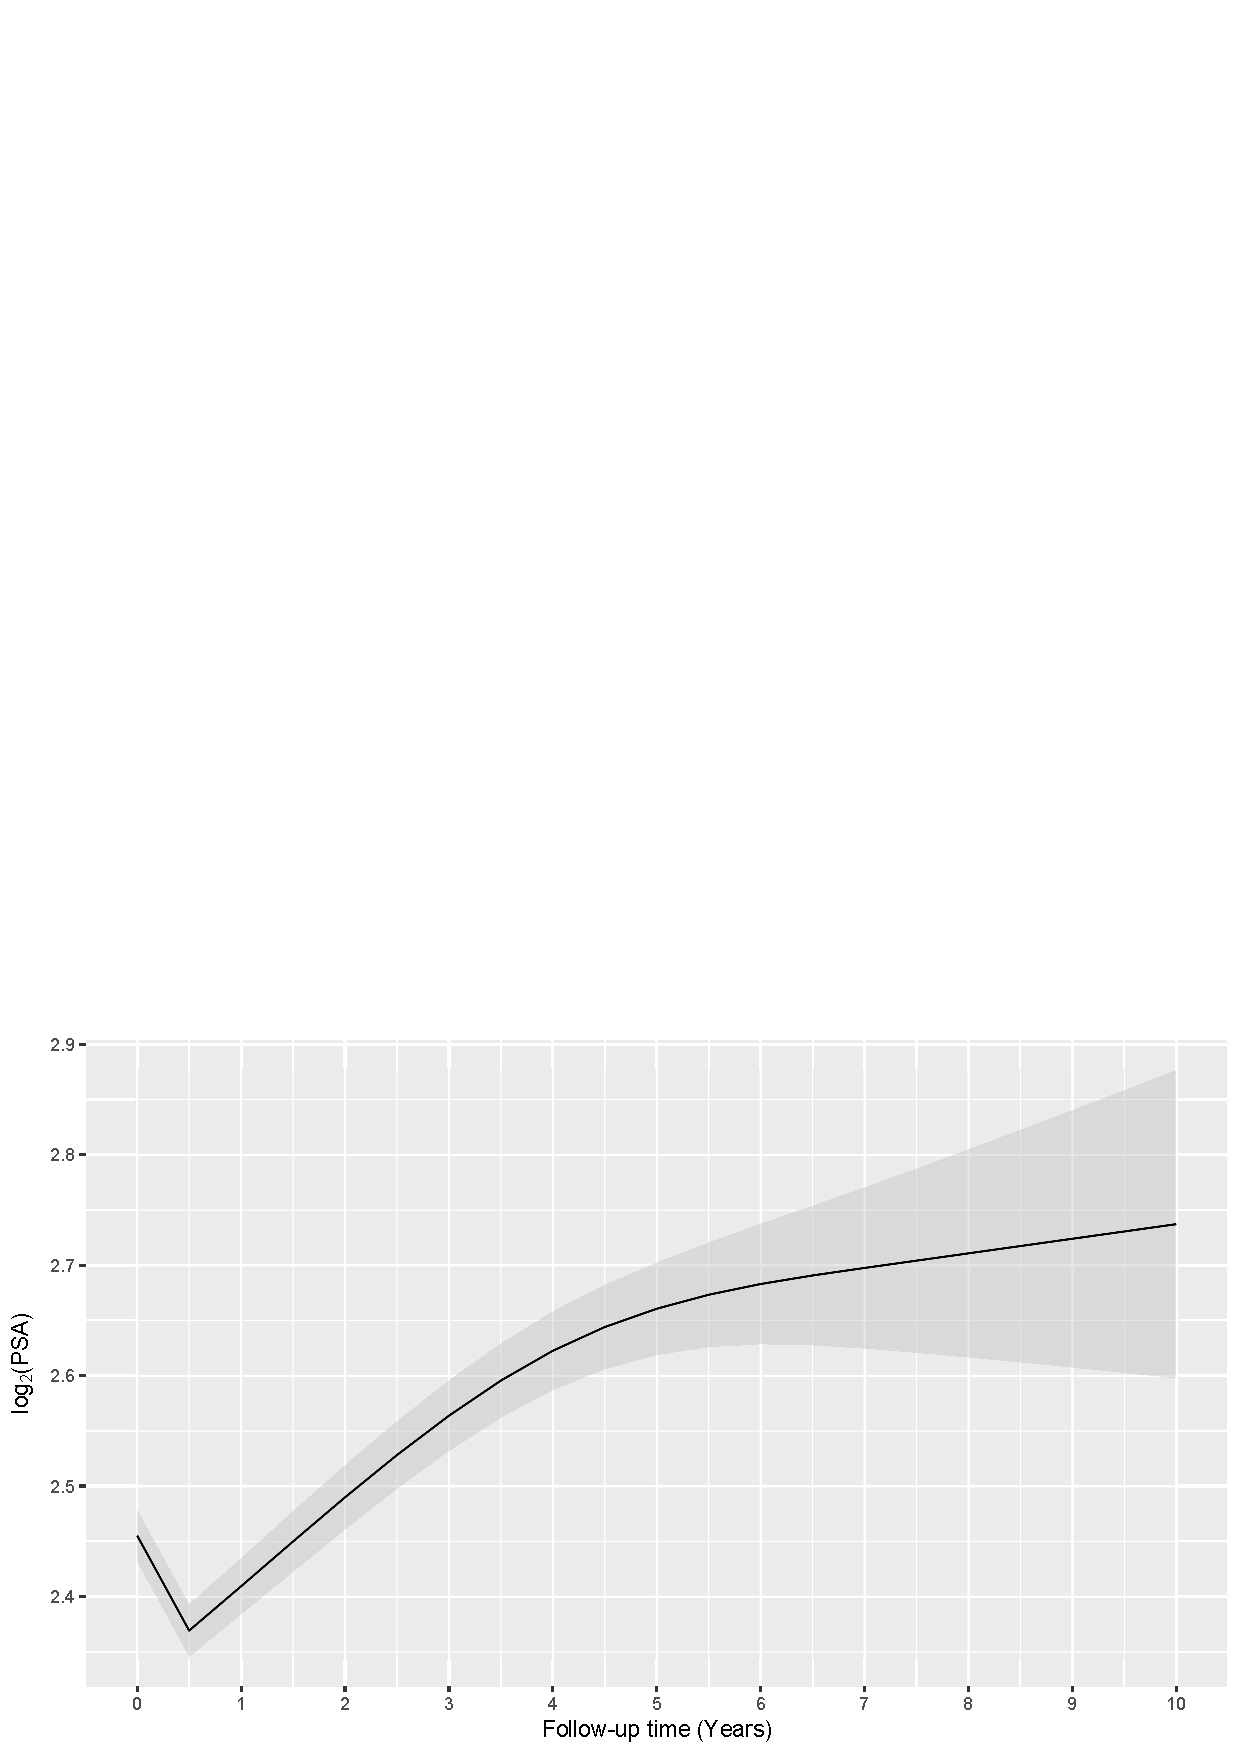
\includegraphics[width=\columnwidth]{images/fitted_trend_psa.png}}
\caption{Fitted evolution of $\log_2 \mbox{PSA}$ over a period of 10 years, for a patient who was inducted in AS at the Age of 70 years.}
\label{fig : fitted_trend_psa}
\end{figure}

\begin{table}
\caption{Longitudinal sub-model estimates for joint model.}
\label{tab : PSA_long}
\begin{tabular}{lrrrrr}
\Hline
& Mean   & Std. Dev           & 2.5\%               & 97.5\%              & P              \\ \hline
Intercept                            &  2.455 & 0.012 & 2.433 & 2.480               & \textless0.000 \\
(Age - 70)                           & 0.003 & 0.001 & 4.9 $\times 10^{-4}$ & 0.006 & 0.032          \\
(Age - 70) $\times$ (Age - 70)       & -0.001 & 1.4 $\times 10^{-4}$ & -0.001 & -3.5 $\times 10^{-4}$ & \textless0.000 \\
Spline: visitTimeYears{[}0, 0.5{]}   & -0.006 & 0.012 & -0.031 & 0.017 & 0.674 \\
Spline: visitTimeYears{[}0.5, 1.2{]} & 0.228 & 0.019 & 0.192 & 0.265               & \textless0.000 \\
Spline: visitTimeYears{[}1.2, 2.5{]} & 0.140 & 0.029 & 0.088 & 0.197               & \textless0.000 \\
Spline: visitTimeYears{[}2.5, 7{]}   & 0.303 & 0.039 & 0.227 & 0.379               & \textless0.000 \\
$\sigma$                               & 0.324 & 0.001 & 0.321 & 0.326              &  \\ \hline
\end{tabular}
\end{table}

\begin{table}
\caption{Survival sub-model estimates for joint model.}
\label{tab : PSA_survival}
\begin{tabular}{lrrrrr}
\Hline
Variable                      & Mean   & Std. Dev & 2.5\%  & 97.5\%                 & P              \\ \hline
Age - 70                      & 0.037 & 0.006 & 0.025 & 0.0490                  & \textless0.000 \\
(Age - 70) $\times$ (Age - 70) & -0.001 & 0.001 & -0.003 & 1.8 $\times 10^{-4}$ & 0.104          \\
$\log_2 \mbox{PSA}$                  & -0.049 & 0.064 & -0.172 & 0.078 & 0.414         \\
Slope($\log_2 \mbox{PSA}$)           & 2.407 & 0.319 & 1.791 & 3.069 & \textless0.000 \\
\hline
\end{tabular}
\end{table}
\clearpage
% !TEX root =  ../supplementary.tex
\section{Additional Examples of Personalized Schedules}
\clearpage
% !TEX root =  ../supplementary.tex
\section{Simulation Study Results}
In the simulation study, we evaluated the following biopsy schedules \citep{loeb2014heterogeneity, inoue2018comparative}: biopsy every year (annual), biopsy according to the PRIAS schedule (PRIAS), personalized biopsy schedules based on two fixed risk thresholds, namely, $\kappa^*=5\%$ and $\kappa^*=10\%$, and automatically chosen $\kappa^*(v)$ (Section~3 of main manuscript), and automatically chosen ${\kappa^*\{v \mid E(D)\leq 0.75\}}$ with a constraint of 9 months (0.75 years) on expected delay in detecting progression. We compare all the aforementioned schedules on two criteria, namely the number of biopsies they schedule and the corresponding time delay in detection of cancer progression, in years (time of positive biopsy - true time of cancer progression). The corresponding results, using ${\mbox{500} \times \mbox{250}}$ test patients are presented in Table \ref{table:sim_study_all}. Since the simulated cohorts are based on PRIAS, roughly only 50\% of the patients progress in the ten year study period. While, we are able to calculate total number of biopsies scheduled in all $500 \times 250$ test patients, but the time delay in detection of progression is available only for those patients who progress in ten years (\textit{progressing}). Hence, we show the simulation results separately for \textit{progressing} and \textit{non-progressing} patients.

\begin{table}[!htb]
\caption{\textbf{Simulation study results for all patients}: Estimated mean, median (Med), first quartile $\mbox{Q}_1(\mbox{nb})$, and third quartile $\mbox{Q}_3(\mbox{nb})$ for number of biopsies and for the delay in detection of cancer progression $\mbox{Q}_1(\mbox{d})$, $\mbox{Q}_3(\mbox{d})$, in years, for various biopsy schedules. The delay is equal to the difference between the time of the positive biopsy and the unobserved true time of progression. Types of schedules: ${\kappa^*=5\%}$, ${\kappa^*=10\%}$ and $\kappa^*(v)$ schedule a biopsy if the cumulative-risk of cancer progression at a visit is more than 5\%, 10\%, and an automatically chosen threshold, respectively. Schedule ${\kappa^*\{v \mid E(D)\leq 0.75\}}$ is similar to $\kappa^*(v)$ except that the euclidean distance is minimized under the constraint that expected delay in detecting progression is at most 9 months (0.75 years). Annual corresponds to a schedule of yearly biopsies, and PRIAS corresponds to biopsies as per PRIAS protocol.}
\label{table:sim_study_all}
\begin{tabular}{l|rrrr|rrrr}
\Hline
\multicolumn{9}{l}{\textbf{Progressing patients (50\%)}}\\
\hline
Schedule & $\mbox{Q}_1(\mbox{nb})$ & $\mbox{Mean}(\mbox{nb})$ & $\mbox{Med}(\mbox{nb})$ & $\mbox{Q}_3(\mbox{nb})$ & $\mbox{Q}_1(\mbox{d})$ & $\mbox{Mean}(\mbox{d})$ & $\mbox{Med}(\mbox{d})$  & $\mbox{Q}_3(\mbox{d})$ \\
\hline
Annual     & 1  & 3.69 & 3  & 6  & 0.29 & 0.55 & 0.57 & 0.82\\
PRIAS      & 1  & 2.87 & 2  & 4  & 0.38 & 0.91 & 0.74 & 1.00\\
$\kappa^*=5\%$  & 1  & 3.30 &  3  & 5  & 0.33 & 0.66 & 0.65 & 0.91\\
$\kappa^*=10\%$ & 1  & 2.55 & 2  & 4  & 0.45 & 1.00 & 0.85 & 1.34\\
$\kappa^*(v)$ & 1  & 2.07 & 2  & 3  & 0.54 & 1.12 & 0.96 & 1.74\\
\hline
\multicolumn{9}{l}{\textbf{Non-progressing patients (50\%)}}\\
\hline
Annual     & 10  & 10 & 10 & 10 & - & - & - & -\\
PRIAS      & 4  & 6.42 & 6  & 8  & - & - & - & -\\
$\kappa^*=5\%$  & 6  & 7.58 & 7  & 9  & - & - & - & - \\
$\kappa^*=10\%$ & 4  & 4.93 & 5  & 6  & - & - & - & - \\
$\kappa^*(v)$ & 3 & 5.47 & 4  & 4  & - & - & - & -\\
\hline
\end{tabular}
\end{table}
%\clearpage
%% !TEX root =  ../supplementary.tex
\section{Source Code}
The R code for fitting the joint model to the PRIAS dataset, and for the simulation study, along with sample dataset, and instructions for running the code are available with this paper at the following link:

\url{https://github.com/anirudhtomer/prias/tree/master/src/decision_analytic}


\clearpage
\printbibliography

\appendix

\end{document}